\documentclass[11pt]{article}
\usepackage{../cs170}


\def\title{Homework 8}
\def\duedate{10/25/2023, at 10:00 pm (grace period until 11:59pm)}

\begin{document}
\maketitle

Due \textbf{\duedate}


\question{Study Group}
List the names and SIDs of the members in your study group.
If you have no collaborators, you must explicitly write ``none''.

\begin{solution}
	None in particular. Received some help in office hours about problem 2 but that's about it.
\end{solution}

\newpage

\question{Egg Drop Revisited}

Recall the Egg Drop problem from Homework 7:
\\\\
\textit{You are given $m$ identical eggs and an $n$ story
building. You need to figure out the highest floor
$\ell \in \{0, 1, 2, \ldots n\}$ that you can drop an egg from without
breaking it. Each egg will never break when dropped from floor $\ell$ or lower, and always breaks if dropped from floor $\ell+1$ or higher. ($\ell = 0$ means the egg always breaks). Once an egg breaks, you cannot use it any more. However, if an egg does not break, you can reuse it.
\\\\
Let $f(n, m)$ be the minimum number of egg drops that are needed to find $\ell$ (regardless of the value of $\ell$).}
\\\\
Instead of solving for $f(n, m)$ directly, we define a new subproblem $M(x, m)$ to be the maximum number of floors for which we can always find $\ell$ in at most $x$ drops using $m$ eggs. 

For example, $M(2, 2) = 3$ because a 3-story building is the tallest building such that we can always find $\ell$ in at most 2 egg drops using 2 eggs.

\begin{subparts}

\item  Find a recurrence relation for $M(x, m)$ that can be computed in constant time given the previous subproblems. Briefly justify your recurrence.

\emph{Hint: As a starting point, what is the highest floor that we can drop the first egg from and still be guaranteed to solve the problem with the remaining $x-1$ drops and $m-1$ eggs if the egg breaks?}

	\begin{solution}
		Here, we use the hint as a basis for our logic, by analyzing what needs to be true whether the egg 
		either breaks or doesn't break. If the egg breaks, then we know that the critical floor is below,
		and we have $x-1$ drops and $m-1$ eggs left. Therefore, in order for us to still be able to solve 
		for \(\ell\), we require that the number of floors below is \(M(x-1, m-1)\). Similarly, if the egg 
		doesn't break, then we know that the critical floor is above us, so we require that the number of 
		floors above us must be \(M(x-1, m)\). Therefore, the maximum height we can solve with \(x\) drops 
		and \(m\) eggs is:
		\[
		M(x, m) = M(x-1, m-1) + M(x-1, m) +1 
		\] 
		Now for our base cases: we know that $M(0, m) = 1$, for any \(m\), since the critical height must exist 
		in the tower, then if the tower is height 1 then we don't need any drops to solve for \(\ell\). 
	\end{solution}
\item  Give an algorithm to compute $M(x, m)$ given $x$ and $m$ and analyze its runtime. 

	\begin{solution}
		Based on our recursion relation, for every subproblem, we have to access two array 
		elements, $M(x-1, m-1)$ and \(M(x-1, m)\), and add them together. This suggests a strategy to create 
		an array of size \(mx\) and solve the problems row by row in increasing \(x\):
		\begin{center}
			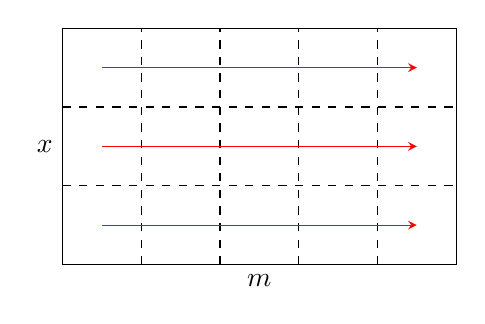
\begin{tikzpicture}
				\draw (0, 0) -- node[midway, below] {\(m\) } (5, 0) -- (5, 3) -- (0, 3) -- node[midway, left] 
				{\(x\) } cycle;
				\foreach \x in {1, 2, 3, 4}
				\draw[dashed] (\x, 0) -- (\x, 3); 
				\foreach \y in {1, 2}
				\draw[dashed] (0, \y) -- (5, \y);
				\foreach \y in {0.5, 1.5, 2.5}
				\draw[-stealth, red] (0.5, \y) -- (4.5, \y);
			\end{tikzpicture}
		\end{center}
		Runtime analysis is in part (d). 
	\end{solution}
\item  Modify your algorithm from (b) to compute $f(n, m)$ given $n$ and $m$.  

\emph{Hint: If we can find $\ell$ when there are more than $n$ floors, we can also find $\ell$ when there are $n$ floors.}

	\begin{solution}
		If we're given \(n, m\), we look through all values of \(M(x, m) = n\), and return the one that 
		has the smallest \(x\) value. This tells us the minimum number of egg drops required to find \(\ell\) 
		with \(x\) egg drops. Mathematically:
		\[
			f(n, m) = \min_{x} \{M(x, m)\ | M(x, m) = n\} 
		\] 
	\end{solution}


\item  Show that the runtime of the algorithm from part (c) is $O(nm)$. Compare this to the runtime you found in last week's homework.

	\begin{solution}
		From part (b) we already know that the runtime to compute each subproblem takes constant time. As 
		for the number of subproblems, we have $O(nm)$ subproblems, one for every \(m\) and also one for 
		every \(n\). Therefore, the total runtime is \(O(nm)\).
	\end{solution}

\item Show that we can implement the algorithm from part (c) to use only $O(m)$ space.

	\begin{solution}
		Looking at our recursion relation, we see that \(M(x, m)\) only depends on the previous row in terms of 
		\(x\). Therefore, this means that to compute \(M(x, m)\) for all \(m\), we only depend on the entries 
		in row \(x-1\). Therefore, we only need \(2m\) space at any given time, meaning that the memory 
		complexity is \(O(m)\).
	\end{solution}

\item Suppose that we are given a special machine that is able to ``revive'' an egg after the first time it breaks so that it is reusable again. In other words, each egg has 2 lives. Based on this modification to the problem, write a new recurrence relation for $M$.

\emph{Hint: you may need to add an additional parameter to your subproblem.}

\begin{solution}
	Because each egg now has two lives, this is the same situation as if each egg has one life, but we doubled 
	the number of eggs since both situations corresponds to the same number of egg breaks. Therefore, the new 
	recursion relation is:
	\[
	M'(x, m) = M(2x, m) = M(2x-1, m) + M(2x-1, m-1) + 1
	\] 
	where \(M'\) is the updated recurrence relation.
\end{solution}
\end{subparts}

\newpage

\question{Knightmare}
Give a dynamic programming algorithm to find the number of ways you can place knights on an $L$ by $H$ ($L < H$) chessboard such that no two knights can attack each other (there can be any number of knights on the board, including zero knights). Knights can move in a \href{https://i.stack.imgur.com/Pebav.png}{$2 \times 1$ shape pattern} in any direction. 

\textbf{Provide a 4-part solution. Your algorithm's runtime should be $O(2^{3L}LH)$, and return your answer mod 1337.}

\begin{solution}

	\textbf{Algorithm Description:} We will define our subproblem by ``growing'' our board column by column from left to right. Let 
	\(f(h, j, k)\) denote the number of ways to arrange knights on a chessboard of height $L$ and width $h$, 
	with $j$ being the second to last row and $k$ being the previous row added. Specifically, the \(i\) and 
	\(j\) here represent the \textit{configuration} of rows $i$ and $j$, not the row indices. Visually: 
	\begin{center}
		\begin{tikzpicture}[scale=0.7]
			\draw (0, 0) -- node[midway, below] {$h$} (10, 0) -- (10, 5) -- (0, 5) --node[midway, left]
				{$L$} cycle;
			\draw[dashed] (9, 0) -- (9, 5);
			\draw[dashed] (8, 0) -- (8, 5);
			\draw[dashed] (7, 0) -- (7, 5);
			\draw node at (7.5, 2.5) {$i$};
			\draw node at (8.5, 2.5) {$j$};
			\draw node at (9.5, 2.5) {$k$};
		\end{tikzpicture}
	\end{center}
	For the recurrence relation, if column \(k\) is the last row that we've added, then the possible 
	arrangements for column \(k \) depend only on rows $i$ and $j$, since knights placed in columns to the left 
	of row $i$ cannot attack any knight placed in row $k$ due to the limitations of the knight's movements. 
	Therefore, we can formulate our recurrence relation as iterating through all configurations for 
	knight placements on column $k$, and check whether the columns $i$ and $j$ satisfy this assignment for $k$. 
	Therefore, we can formulate the recursion as, for a given arrangement of $k$:
	\[
		f(h, j, k) = \sum_{\text{satisfying \(i, j\)}} f(h-1, i, j) \pmod{1337}
	\] 
	As for our base cases, $f(1, i, j) = 2^L$, since any configuration of knights on a \(1 \times L\)
	chessboard is a valid configuration.

	Finally, here's the order in which we solve the subproblems.   
	Because we're defining the subproblems in this way, then it makes sense that the order in which we should 
	solve them is starting with $h = 0$, then ``growing'' the board until we get a width of $H$.  

	\textbf{Proof of Correctness:} To prove that this is correct, we just have to prove that the search is 
	exhaustive. Firstly, the base case of $f(1, i, j) = 2^L$ is correct since any configuration of knights 
	is a valid configuration on a \(1 \times L\) chessboard. Now, assume that all \(f(h-1, i, j)\) have 
	been computed. This means that all valid configurations of knights in rows \( i\)and \(j\) have been 
	computed. Now, the recurrence relation says that for every configuration of $k$, we look at 
	which configurations of \(i, j\) satisfy this configuration of \(k\). Since this process 
	looks at every configuration \(f(h-1, i, j)\), once it finds a valid configuration, we add it to 
	\(f(h, j, k)\), and since the search of \(k\) is exhaustive, then the whole search is as well by induction.

	Finally, taking this modulo 1337 at every step is also valid, since it doesn't matter the order in which 
	we add and take modulo 1337. 

	\textbf{Runtime Analysis:} This is determined by the number of subproblems, and the work done at every 
	subproblem. Based on our subproblem definition, the number of subproblems is given by the total number 
	of configurations for columns \(i, j\), then multiplied by $H$ since there are $H$ columns in total. For 
	the columns \(i, j\), there are $L$ squares in each column, and both columns are independent of one another, 
	so there are \(2^L \times  2^L = 2^{2L}\) configurations for columns \(i\) and \(j\). Therefore, there are
	in total \(2^{2L} \cdot H\) subproblems.

	At every subproblem. we are running through all the possible arrangements for the knights in column \(k\), 
	which there are also \(2^L\) of. Furthermore, the process of checking whether an assignment is valid can 
	be done in \(O(L)\) time, since all we need to check are whether the knights in column \(k\) attack any of 
	the knights in column \(i\) and \(j\). Therefore, the work per subproblem is \(O(2^{L} \cdot L\). 
	Therefore, the total runtime is:
	\[
		O(2^{2L} \cdot H) O(2^L \cdot L) = O(2^{3L}LH)
	\] 
	as desired. 


	\textbf{Space Analysis:} Notice that at every \(f\), we only care about $f(h-1, i, j)$ for rows \(i\) and 
	\(j\). This means that in reality, we only need to keep track of two rows at a time: $f(h, j, k)$ and 
	\(f(h-1, i, j)\). In terms of space complexity, there are three rows through which we're iterating through 
	combinations, so this means that there are \(2^{3L}\) total combinations we need to keep track of, 
	and hence we have a space complexity of \(O(2^{3L})\).
\end{solution}

\newpage

\question{Max Independent Set Again}

You are given a connected tree $T$ with $n$ nodes and a designated root $r$, where every vertex $v$ has a weight $A[v]$. A set of nodes $S$ is a $k$-independent set of $T$ if $|S| = k$ and no two nodes in $S$ have an edge between them in $T$. The weight of such a set is given by adding up the weights of all the nodes in $S$, i.e. 
\[w(S) = \sum_{v \in S} A[v].\] Given an integer $k \leq n$, your task is to find the maximum possible weight of any $k$-independent set of $T$. We will first tackle the problem in the special case that $T$ is a binary tree, and then generalize our solution to a general tree $T$.

\begin{subparts}
    \item Assume that $T$ is a binary tree, i.e. every node has at most 2 children.  Describe an $O(nk^2)$ algorithm that solves this special case, and analyze its runtime. Proof of correctness and space complexity analysis are not required.

		\begin{solution}
			Let $T(n, r, f)$ be the max \(n\)-dependent set of a tree rooted at \(r\), and \(f\) being a flag 
			denoting whether the root node was included in the set or not. \(f = 1\) means that 
			the root was included, and \(f= 0\) denotes that it was excluded. Given this, we can calculate 
			two things:
			\begin{align*}
				T(m, r, 1) &= \max_{L, R} \{T(m-i-1, L, 0) + T(i-1, R, 0) \ | i \in \{1, \dots, k\} \} + A[r]\\
				\begin{split}
				T(m, r, 0) &= \max_{L, R} \{T(m-i, L, 1) + T(i, R, 1), 
				T(m-i, L, 0) + T(i, R, 0), \\ & T(m-i, L, 1) + T(i, R, 0), T(m-i, L , 0) + T(i, R, 1) \ | i \in \{0, \dots, k\} \}  
				\end{split}
			\end{align*}
			We need to do this for all $m = 1, \ldots, k$ so that we can recurse upwards. 

			As for the logic, we're looking for combinations of independent sets of the children such that the 
			union of these two sets is of size \(m\). For \(T(m, r, 1)\), we are choosing the root (indicated
			by \(f = 1\) ), so 
			we need to choose $T$ such that the children aren't included, so their flags 
			must be zero. Further, note that in this case we require that the number of elements selected 
			in the children is $m-1$, since we need to include the root node. We then select the maximum 
			of these sets, which tells us the optimal \(k\)-independent set. 

			Similar logic is used for \(T(n, r, 0)\), where we're now allowed to include the 
			children. However, because we \textit{don't have to include the children}, 
			we have to take the max over 
			the instances where the child node is selected and also include instances where the child node 
			isn't selected. This corresponds to the flags being in the set: \((1, 1), (0, 0), (0, 1), (1, 0)\).
			This is also why the second line is so much longer, since we have more cases to handle. 
			
			As for the base cases, if the node is a leaf then $T(i, r, 1) = A[r]$, and $T(i, r, 0) = 0$ for all 
			\(i \in \{1, 2, \dots, k\} \).

			\textbf{Runtime Analysis:} First, let's look at the work per subproblem. At every subproblem, we are
			checking \(O(k)\) array entries (assuming that we're memoizing using an array), so this is \(O(k)\) 
			work with every subproblem. Then, for every node, there are \(O(k)\) subproblems, one for each 
			\(m\)-independent set rooted at that node. This makes a total of \(O(nk)\) subproblmes, for a total 
			runtime of \(O(nk^2)\).
		\end{solution}
    \item Now, consider any arbitrary tree $T$, with no restrictions on the number of children per node. Describe how we can add up to $O(n)$ ``dummy'' nodes (i.e. nodes with weight 0) to $T$ to convert it into a binary tree $T_b$. 

		\begin{solution}
			For every node with greater than 2 children, we select all but one of its children, then 
			introduce a dummy node that connects their common ancestor with the unselected node. Visually, 
			it looks like this:
			\begin{center}
				\begin{tikzpicture}[level distance=20mm]
					\node {A}	
						child {node{B}}
						child {node {C}}
						child {node {D}};
				\end{tikzpicture}
				\begin{tikzpicture}
					\draw[-stealth] (0, 1.1) -- (3, 1.1);
					\draw[white] (0,0) circle (0.001cm);
				\end{tikzpicture}
				\begin{tikzpicture}[level distance = 10mm]
					\node {A} 
						child {node {B}}
						child {node [red]{0}
							child {node {C}}
							child {node {D}}
						};
				\end{tikzpicture}
			\end{center}
			In this case, we can stop here since this is now a binary tree. However, if there are more 
			than 2 children connected to the dummy node, we can repeat this process until all nodes have 
			at most 2 children. This process is repeated at most \(O(n)\) times, once for every node, so 
			we add at most \(O(n)\) dummy nodes. 
		\end{solution}

    \item Using your responses to parts (a) and (b), describe an $O(nk^2)$ algorithm to solve the general case (i.e. when $T$ is any arbitrary tree), and analyze its runtime. Proof of correctness and space complexity analysis are not required.

		\begin{solution}
			Here, we can use the same process as part (a), but modify our algorithm for the case where 
			we're at a dummy node. In this case, we want the flag for the dummy node to be the same 
			as the flag for its children, since by selecting the dummy node we want it to encode the fact that 
			we are selecting the children and vice versa. 

			Recall that in our recursion relation in part (a), we search through the children with flag 
			\(0\) when the parent node is selected, meaning that from the perspective of our dummy node, 
			a flag of 0 means that we cannot select any of its children (since the children were adjacent 
			to the dummy's parent in the original graph). On the other hand, a flag of 1 means that we are 
			allowed to select the children, so in total the following is our recursion relation:  
			\begin{align*}
				T(n, r_d, 0) &= \max_{L, R} \{T(n-i, L, 0) + T(i, R, 0) \ | 
				i \in \{0, \dots, k\} \}\\
				\begin{split}
				T(n, r_d, 1) &= \max_{L, R} \{T(n-i, L, 1) + T(i, R, 1), T(n-i, L, 1) + T(i, R, 0), 
						 \\	&T(n-i, L, 0) + T(i, R, 1), T(n-i, L, 0) + T(i, R, 0) \ | i \in \{0, \dots, k\} 
					\} 
					\end{split}
			\end{align*}
			for all \(n \in \{1, \dots, k\}\). Note that since we have a maximum of \(O(n)\) dummy 
			nodes, there are maximally \(O(2n)\) nodes in our graph, which doesn't hurt the runtime 
			we derived in part (a). Therefore, the runtime for this algorithm is also \(O(nk^2)\).
		\end{solution}
\end{subparts}

\newpage

\question{Coding Questions}

For this week’s coding questions, we'll implement dynamic programming algorithms to solve two classic problems: \textbf{Weighted Independent Set in a Tree} and \textbf{TSP}.  There are two ways that you can access the notebook and complete the problems:
\begin{enumerate}
    \item \textbf{On Local Machine}: \texttt{git clone} (or if you already cloned it, \texttt{git pull}) from the coding homework repo, 
    
    \textcolor{blue}{\href{https://github.com/Berkeley-CS170/cs170-fa23-coding}{\texttt{https://github.com/Berkeley-CS170/cs170-fa23-coding}}}
    
    and navigate to the \texttt{hw08} folder. Refer to the \texttt{README.md} for local setup instructions.

    \item \textbf{On Datahub}: Click \textcolor{blue}{\href{https://datahub.berkeley.edu/hub/user-redirect/git-pull?repo=https://github.com/Berkeley-CS170/cs170-fa23-coding}{here}} and navigate to the \texttt{hw08} folder if you prefer to complete this question on Berkeley DataHub.
\end{enumerate}

\noindent Notes:
\begin{itemize}
    \item \textit{Submission Instructions:} Please download your completed submission \texttt{.zip} file and submit it to the Gradescope assignment titled ``Homework 8  Coding Portion''.
        
    \item \textit{OH/HWP Instructions:} Designated coding course staff will provide conceptual and debugging help during office hours and homework parties.

    \item \textit{Edstem Instructions:} Conceptual questions are always welcome on the public thread. If you need debugging help first try asking on the public threads. To ensure others can help you, make sure to:
        \begin{enumerate}
            \item Describe the steps you've taken to debug the issue prior to posting on Ed.
            \item Describe the specific error you're running into.
            \item Include a few small test cases, alongside both the output you expected to receive and your function's actual output. 
        \end{enumerate}
    If staff tells you to make a private Ed post, make sure to include \textit{all of the above items} plus your full function implementation. If you don't provide them, we will ask you to provide them.
    
    \item \textit{Academic Honesty Guideline:} We realize that code for some of the algorithms we ask you to implement may be readily available online, but we strongly encourage you to not directly copy code from these sources. Instead, try to refer to the resources mentioned in the notebook and come up with code yourself. That being said, we \textbf{do acknowledge} that there may not be many different ways to code up particular algorithms and that your solution may be similar to other solutions available online.
    
\end{itemize}
\end{document}
